\subsection{System Analysis}

The development process begins with a thorough analysis of the TTGO T-Display ESP32 board, which serves as the core component of the system. This phase involves a detailed inspection of the board's physical dimensions, including its overall footprint, the positions of connectors, buttons, and the integrated display, as well as any protrusions that must be accommodated by the enclosure.

\begin{figure}[H]
    \centering
    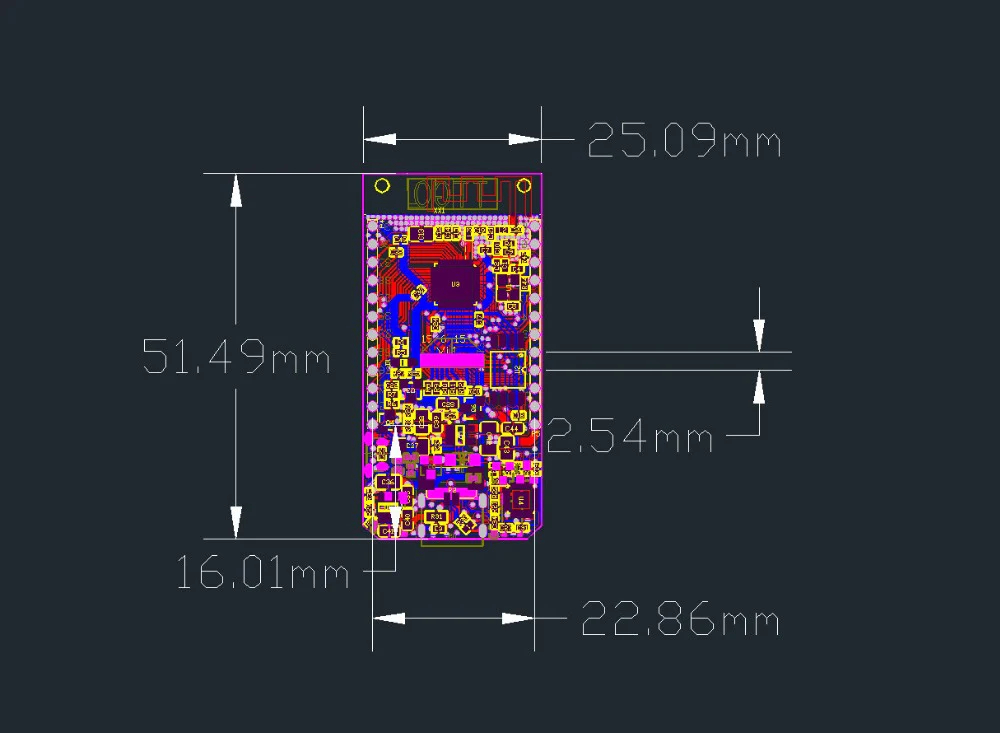
\includegraphics[width=0.5\textwidth]{development-testing/development/image/esp32ttgo_dimension.png}
    \caption{TTGO T-Display ESP32 board dimensions.}
    \label{fig:esp32ttgo_dimension}
\end{figure}

Alongside the dimensional study, the board's architectural specifications are reviewed:

\begin{itemize}
    \item The ESP32 dual-core microcontroller
    \item The 1.14-inch ST7789V TFT display
    \item The USB-C charging interface
    \item The LiPo battery connector
\end{itemize}

\begin{figure}[H]
    \centering
    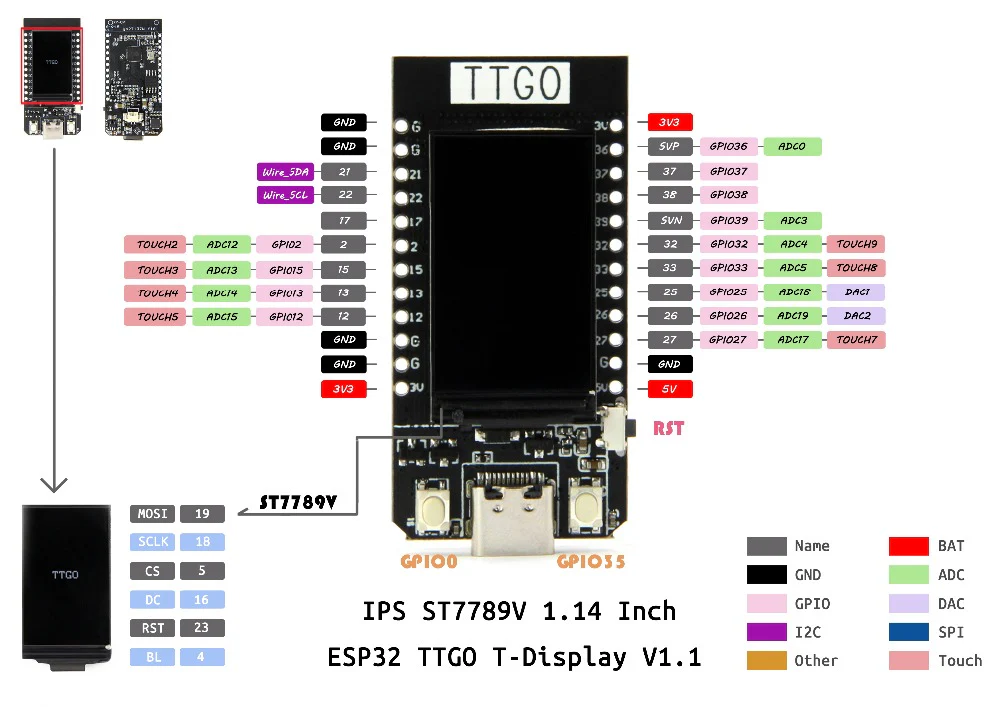
\includegraphics[width=1\textwidth]{development-testing/development/image/esp32ttgo_specification.png}
    \caption{TTGO T-Display ESP32 board specifications.}
    \label{fig:esp32ttgo_specification}
\end{figure}

The outputs of this phase directly constrain the mechanical design: every internal cavity, port cutout, and mounting feature in the housing must correspond to the physical layout established here. System analysis therefore acts as the foundational step that ensures dimensional accuracy and functional compatibility throughout the rest of the pipeline.